\begin{frame}
  \frametitle{Sillabificazione - Metodi}
  \begin{columns}
    \begin{column}{0.4\textwidth}
      Il metodo basato sulla \textbf{sonorità} ha permesso
      di ridurre le dimensioni del codice del \textbf{65\%},
      e di rendere il sillabificatore generico sull'\textit{input}
    \end{column}
    \begin{column}{0.4\textwidth}
      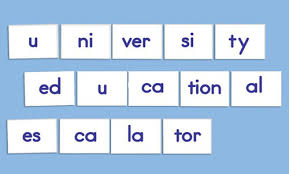
\includegraphics[width=1\columnwidth]{syllabification.jpg}
    \end{column}	
  \end{columns}
\end{frame}
